
% Due thursday

\documentclass{article}

\usepackage[utf8]{inputenc}

\usepackage{amsmath, bm}
\usepackage{graphicx}
\usepackage{amssymb}
\usepackage{float}
\usepackage{caption}
\usepackage{subcaption}
\usepackage{hyperref}
\usepackage{tikz}
\usepackage{layout}

\usepackage[margin=1in]{geometry}
\usepackage{listings}
\usepackage{xcolor}
\usepackage{color, colortbl}
\usepackage{textgreek}
\usepackage{mathrsfs}
\usepackage{savetrees}


\setlength{\parskip}{\baselineskip}%
\setlength{\parindent}{0pt}%
\linespread{0.9}


\definecolor{codegreen}{rgb}{0,0.6,0}
\definecolor{codegray}{rgb}{0.5,0.5,0.5}
\definecolor{codepurple}{rgb}{0.58,0,0.82}
\definecolor{backcolour}{rgb}{0.95,0.95,0.92}

\lstdefinestyle{mystyle}{
    backgroundcolor=\color{backcolour},   
    commentstyle=\color{codegreen},
    keywordstyle=\color{magenta},
    numberstyle=\tiny\color{codegray},
    stringstyle=\color{codepurple},
    basicstyle=\ttfamily\footnotesize,
    breakatwhitespace=false,         
    breaklines=true,                 
    captionpos=b,                    
    keepspaces=true,                 
    numbers=left,                    
    numbersep=5pt,                  
    showspaces=false,                
    showstringspaces=false,
    showtabs=false,                  
    tabsize=2
}

\lstset{style=mystyle}



\begin{document}

\title{GA3: Heat Exchanger Final Report}
\author{lwp26 Group E}
\date{June 2024}
\maketitle 


\section{Introduction}

The development of heat exchanger design software is incomplete without real world performance evaluation.
This report covers the assembly, testing and final performance of the assembled design chosen by our software compared to those selected and built by other groups.

\section{Results}

\subsection{Group E Assembly}
A major design flaw appeared due to not considering a 1mm gap for the outer O ring between inner and outer shell lengths which forced use to increase tube length by 3mm.
Another small issue was that the compression cage did not allow the the nozzles to be 60 degrees apart, as specified by the drawings. This was easily fixed by rotating the nozzles and outer shells slightly
out of alignment with the inner tube passes.
The diameter for small O rings and tubes was 0.36mm smaller than the value of 10.92 mm defined in the handout which was caused by instead defining the angle to be 45 degrees, which was not the case.
This issue made it harder to assemble the tubes, but also provided a better seal between cold and hot sections.
% nozzle problems
% baffle and end cap assembly problems

\begin{figure}[H]
    \centering
    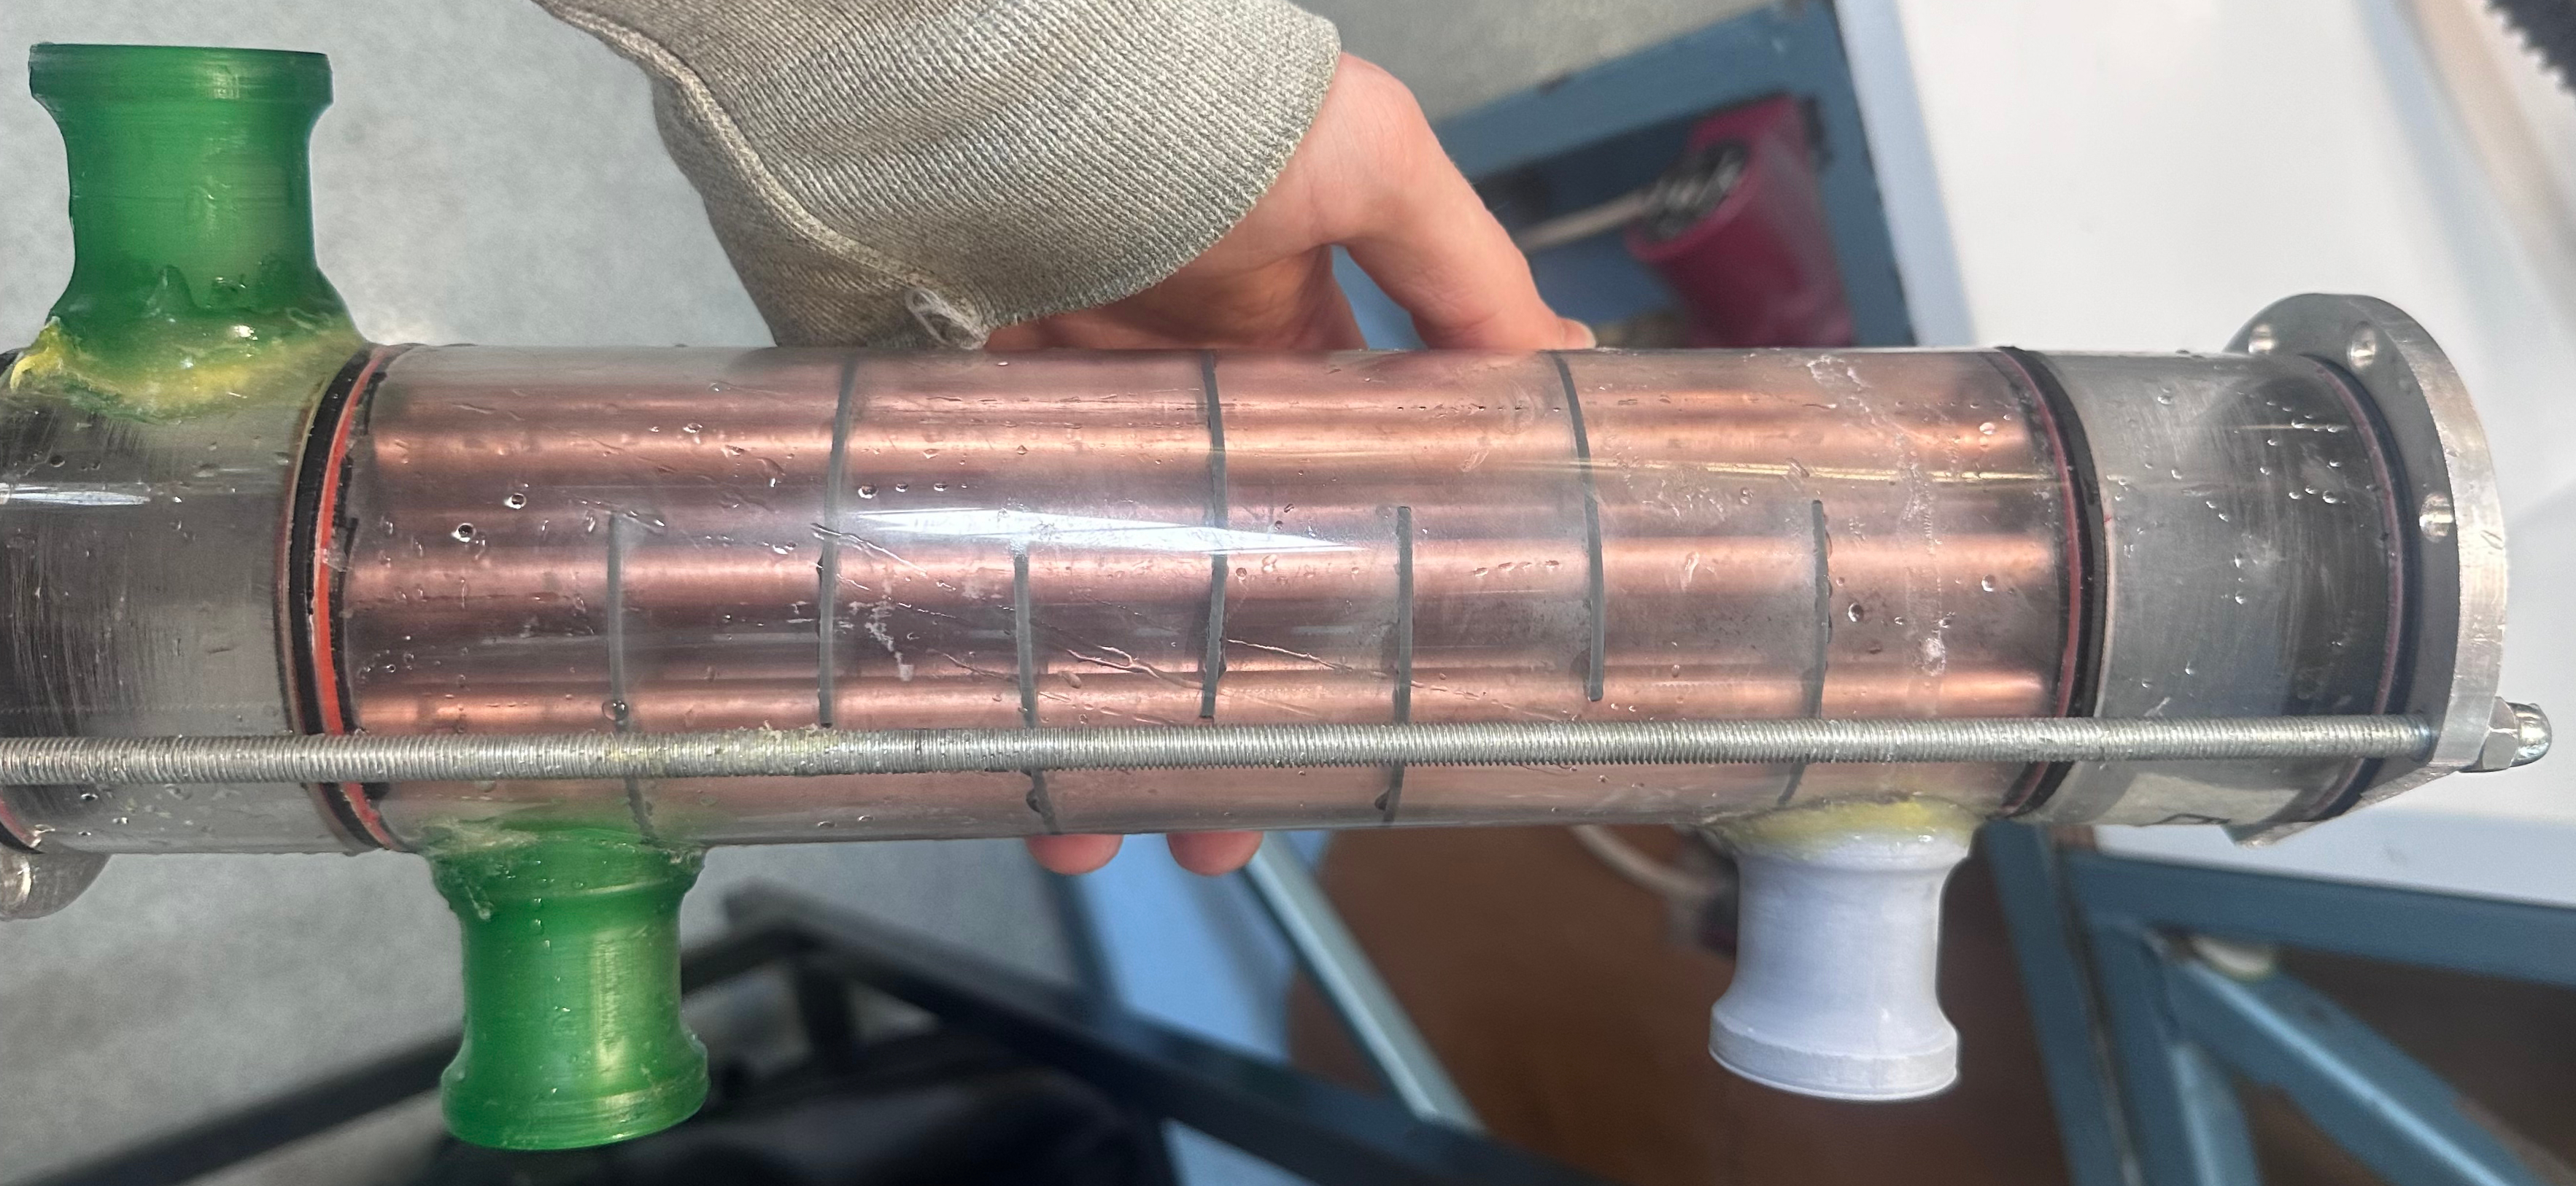
\includegraphics[width=0.5\textwidth]{final_tested.jpg}
    \caption{Final tested heat exchanger}
    \label{fig:heat_exchanger}
\end{figure}

These issues immidiately highlight differences which were not accounted for in the uncertainty analysis in the previous performance report.
Other groups may have also made small changes due to unforeseen issues, which could have affected the performance of their heat exchangers.

\section{Results}

\iffalse
\begin{figure}[H]
    \centering
    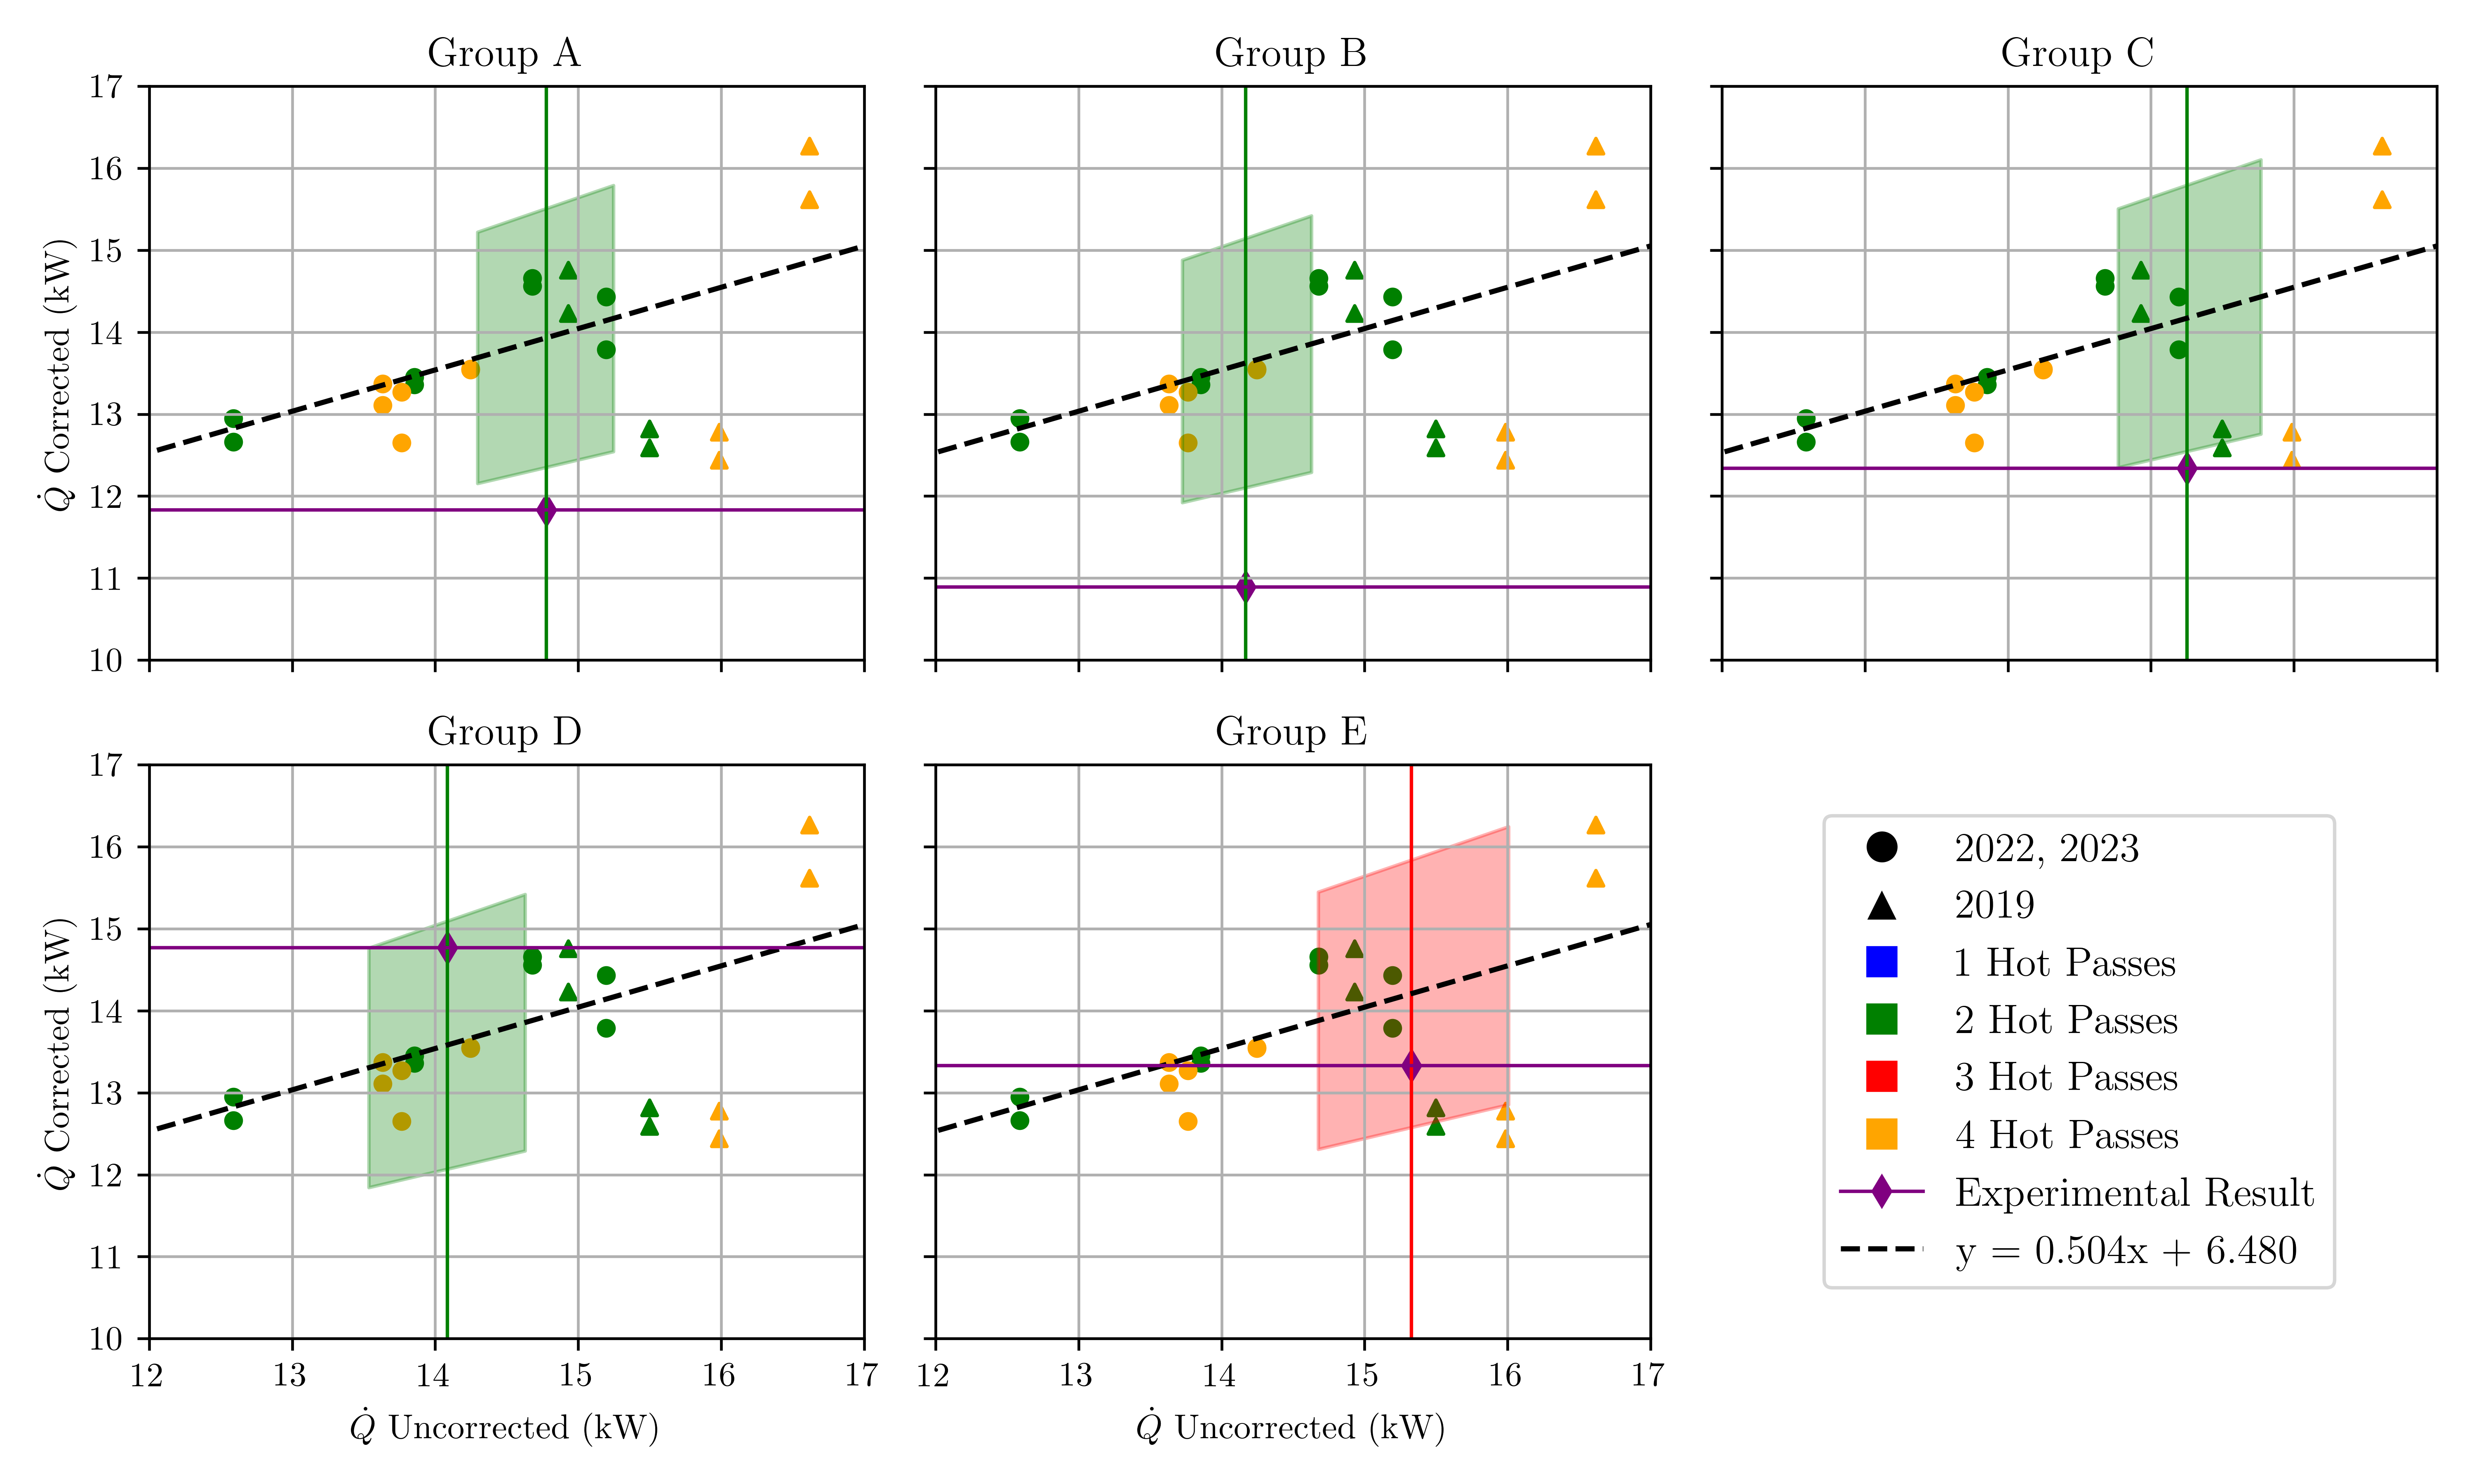
\includegraphics[width=0.9\textwidth]{Qdot_result_bands.png}
    \caption{Qdot results}
    \label{fig:Qdot_results}
\end{figure}
\fi

\begin{figure}[H]
    \centering
    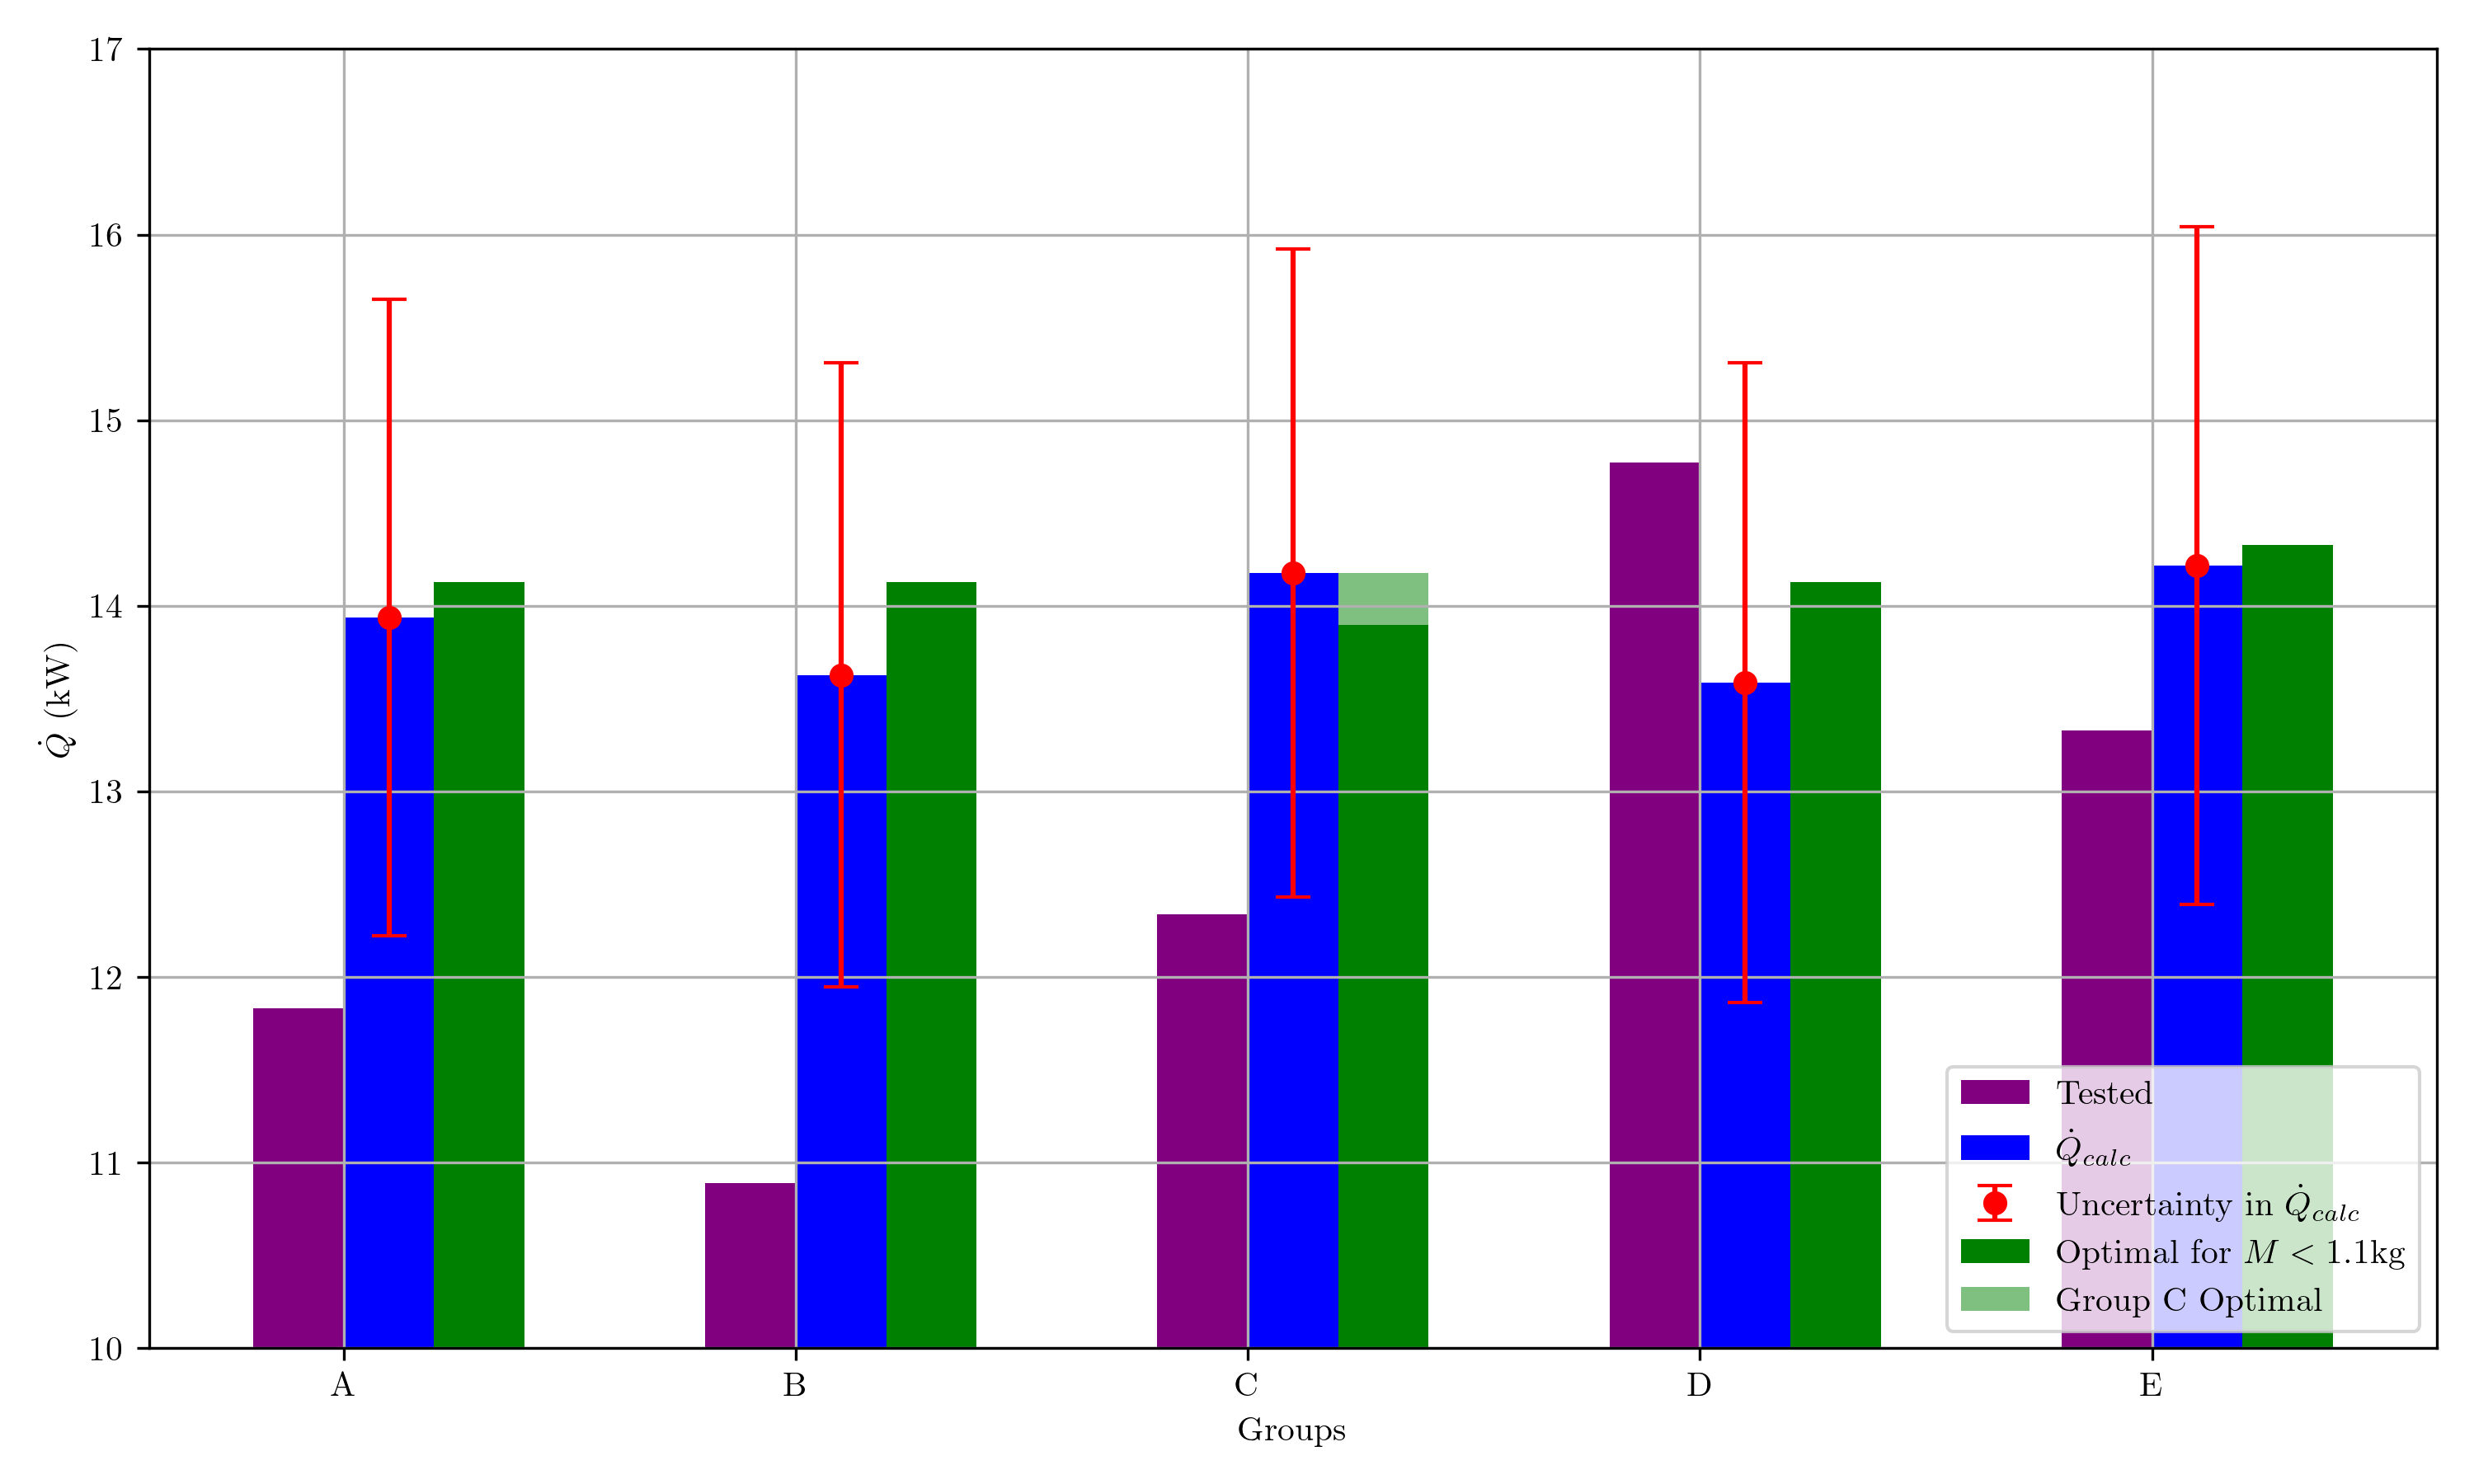
\includegraphics[width=0.6\textwidth]{2024_results.png}
    \caption{$\dot{Q}$ results}
    \label{fig:Qdot_results} 
\end{figure}

\begin{figure}[H]
    \centering
    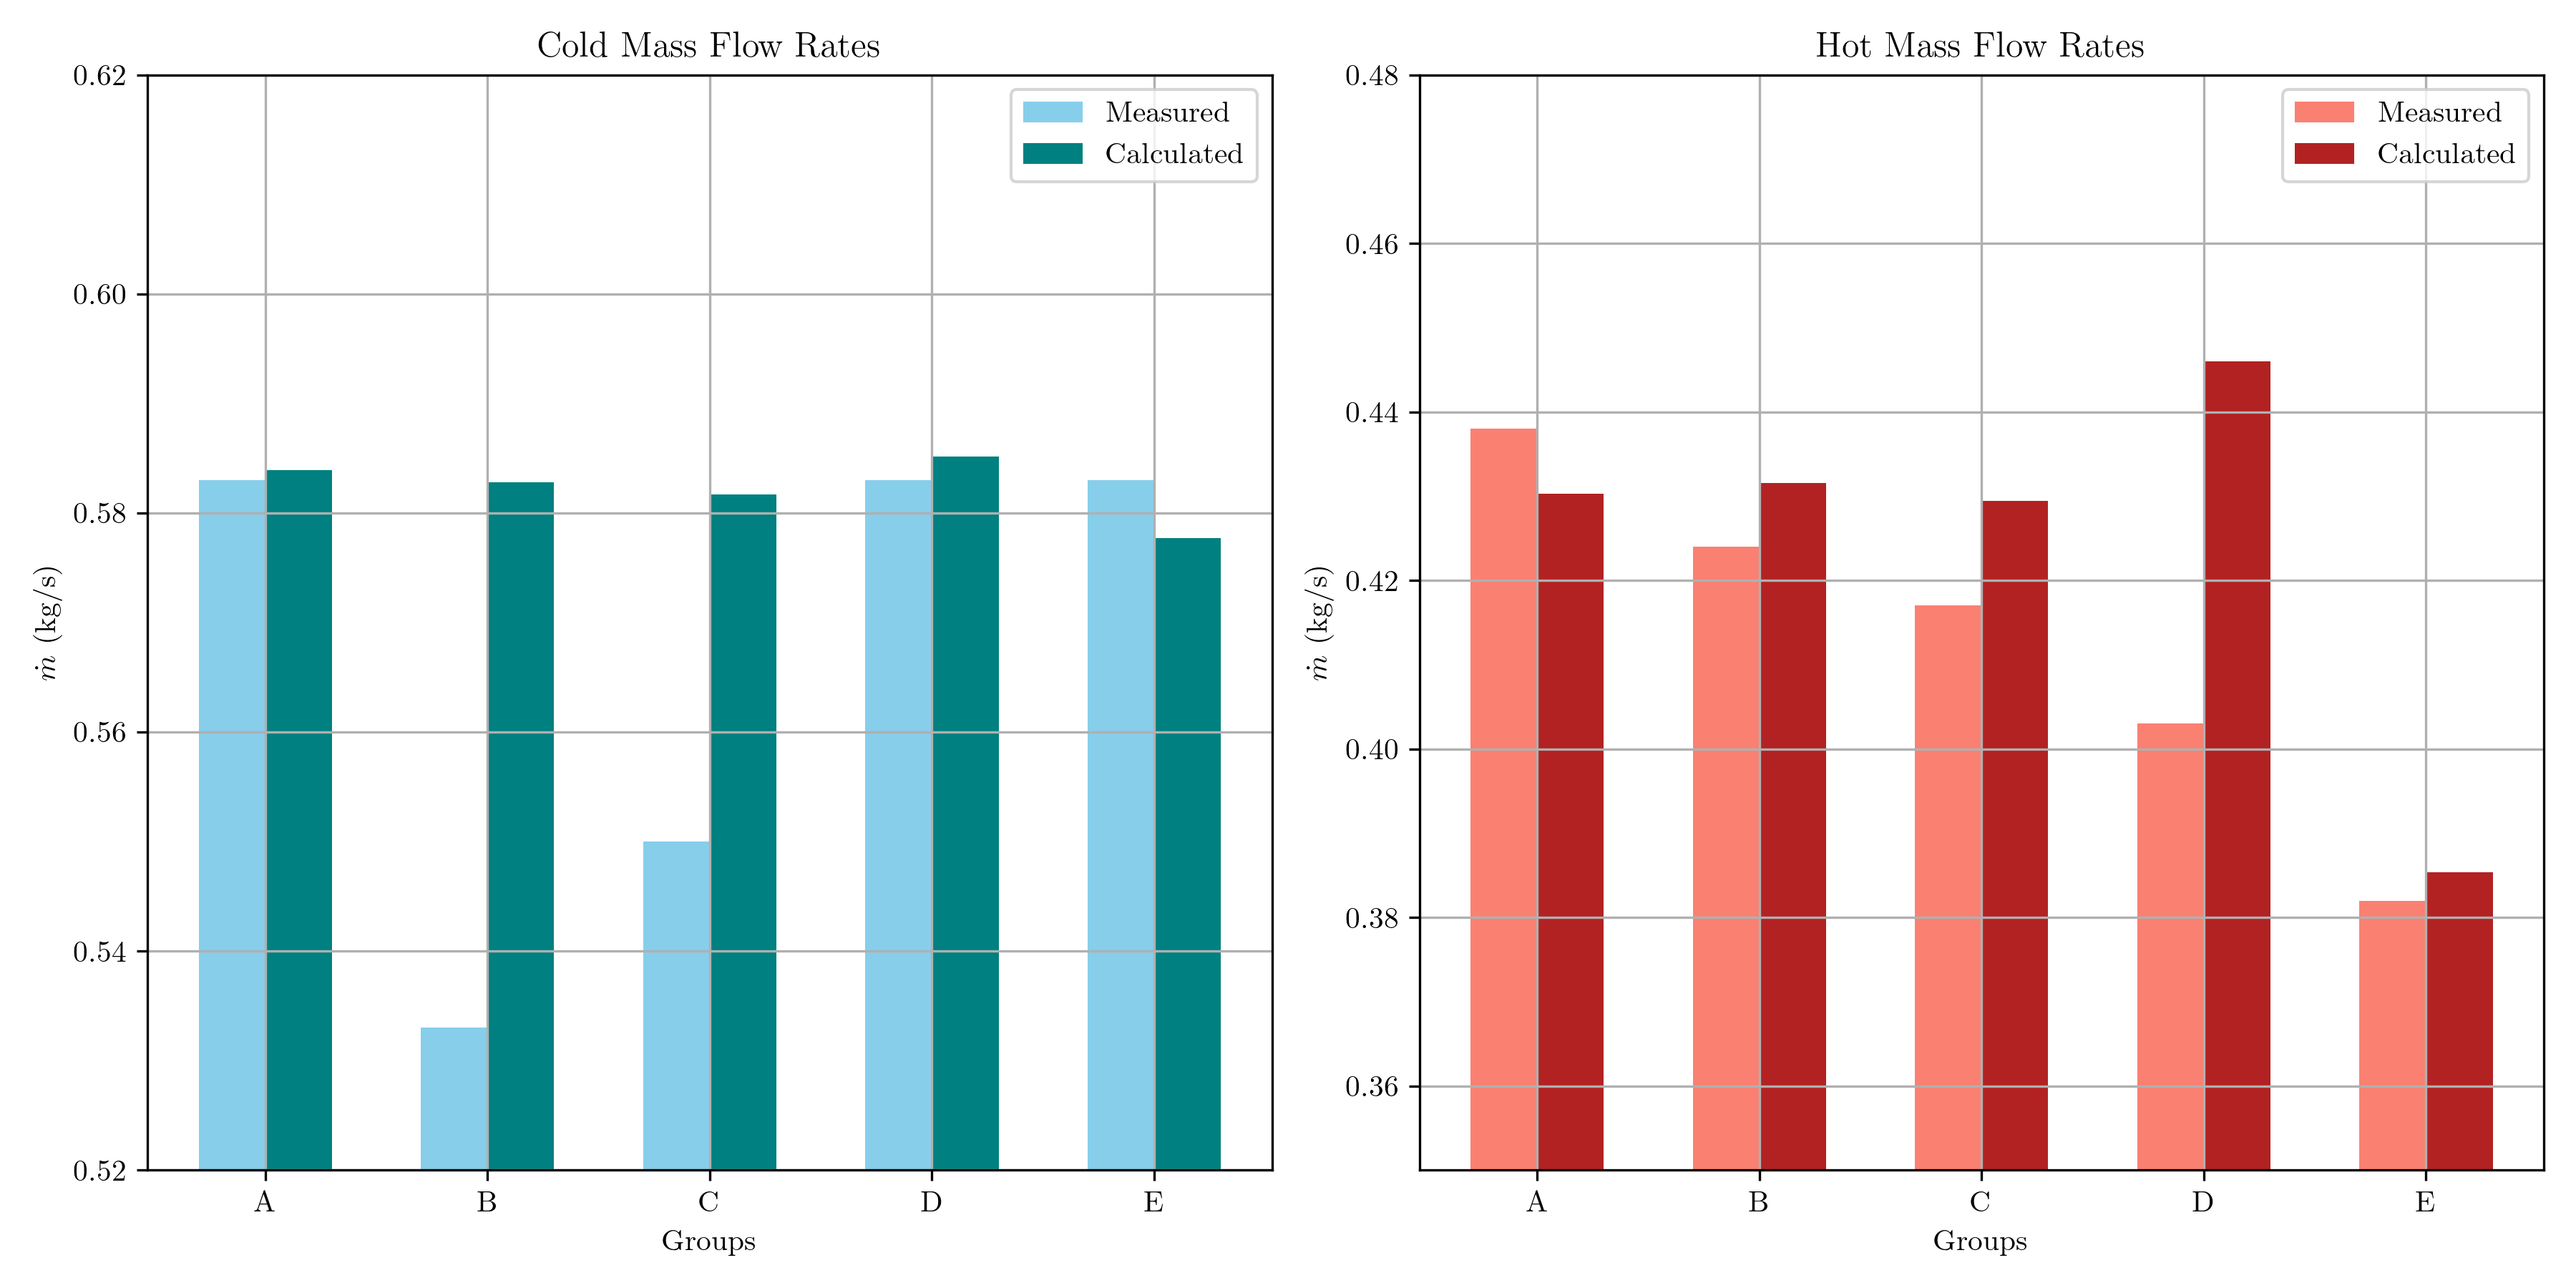
\includegraphics[width=0.7\textwidth]{2024_mass_flow_rates.png}
    \caption{Mass flow rates of hot and cold sides for each group}
    \label{fig:mdot_results}
\end{figure}

Figure \ref{fig:Qdot_results} shows the experimental results for the heat exchanger performance of each group.
Group D's heat exchanger performed the best at 14.77 kW, exceeding our calculated value by 8.7\%, but within the uncertainty band of 12.69\%.
Our group E heat exchanger had the second best performance 9.7\% below that of Group D, and 6.2\% below our calculated value.
The remaining groups ranked C, A and then B at 16.5\%, 19.9\% and 26.3\% below group D, which is the same order predicted by our software.
Figure \ref{fig:Qdot_results} also shows that these last 3 groups are outside of the uncertainty bands with experimental values being
-13.0\%, -15.1\% and -20.1\% below the respective calculated values.
% explain discrepency in B and C using poorly calculated cold mass flow rates due to kerns method again
% A is hard to explain as mass flow rates agree with calculations they did leak though
% comment on group C hot flow being lower than expected due to underestimating pressure drop of their special manifold


The experimental and calculated mass flow rates for both hot and cold sides are shown in Figure \ref{fig:mdot_results}.
This shows that the cold mass flow rates for groups B and C were predicted to be 8.5\% and 5.5\% lower than calculated values.
Kerns method is known to underestimate the pressure drop, which could be the cause of this, however groups A, D and E cold mass flows were all within 1\% of their calculated values.
Another possible cause is that group B had long thin 'baffle spacers' which could have caused a larger pressure drop than expected.
Group C was the only design to have two cold shell passes, which may underestimate the pressure drop from flow reversal in the U bend.
Uncertainty analysis in mass flow rates was not conducted but the addition of two shell side pressure drops will give a higher propagated uncertainty than the other groups.
Group A performs outside of the uncertainty band, despite having hot and cold mass flow rates within 2.3\% of the calculated values.
It was also noted that group A had a leak in their heat exchanger, which indicate that the actual mass flow is lower on the side that leaked,
causing a reduction in performance.


% more detailed fouling, comparison with bell delaware method
% additional constraints and design considerations for variety of applications:
% - optimal performance at a range of operating conditions
% - robustness to fouling and ease of maintenance
% - cost of materials and manufacturing at scale
% - ease of assembly and disassembly
% software improvements

\section{Recommendations}
% hard section to write
% a 3-1 configuration is recommended for this application
% despite textbooks stating that an odd number of hot passes 
% with more counterflow passes than coflow passes may result in structural and thermal problems
An odd number of hot passes, with more counterflow passes than coflow passes, has a slightly better effectiveness
than an even number of hot passes with an equal number of coflow and counterflow.
Textbooks state these uncommon designs may result in structural and thermal problems \cite{HeatTransfer}.
However for this application of compact heat exchangers, the lengths and operating temperature gradients are small so thermal expansion is negligible.
An additional hot pass comes at a cost of increased pressure drop compared to a smaller number of even hot passes, however the increased effectiveness was found to be worth the tradeoff.
% However, this is an uncommon design and may result in structural and thermal problems in manufacturing and design.

% tube count and position and length
Tube count, position and length are the most important factors in determining the heat exchanger performance.
Increasing heat transfer area will generally increase the heat transfer rate and can be done by increasing tube count or length.
However this needs to be done carefully as increasing the length increases the hot side pressure drop, increasing tube count reduces hot side pressure drop but increases cold side pressure drop.
Table 1 of the Interim Report \cite{InterimReport} shows optimized lengths and tube counts for a variety of heat exchanger configurations.
The software also recommended longer designs with more tubes in later hot passes over shorter designs with an equal number of tubes in each hot pass.
This is because increasing the heat transfer area at regions of smaller temperature differences increases the overall heat transfer.

% baffle count
Increasing baffles increases the cold side pressure drop, decreasing the mass flow rate,
however, it also increases the shell side Nusselt number, and therefore the overall heat transfer coefficient.
For a given design there is a point at which the increased heat transfer coefficient is outweighed by the reduction in mass flow rate.
Kerns method seemed to overestimate this optimal number of baffles, selecting designs with $\sim20$ baffles.
This makes it difficult to recommend this method for selecting the optimal number of baffles and a more detailed Bell-Delaware method should be considered instead.
Our group chose to add a constraint such that the baffle spacing was more than half the shell diameter,
however due to thickness and nozzle placement, the actual baffle spacing was reduced.

\section{Future Work}

\begin{itemize}
    \item Implementing Bell-Delaware method with a detailed comparison Kerns method for more accuate shell side pressure drop calculations.
    \item Additional constraints and design considerations could be considered for additional applications:
    \begin{itemize}
        \item Optimizing the heat exchanger performance over a range of inlet temperatures or compressor characterisitcs.
        \item Enhancing the design's robustness to fouling and ease of maintenance to minimize costs and extend the heat exchanger's lifespan.
        \item Considering the cost of materials and manufacturing at scale of the designed heat exchangers.
    \end{itemize}

    \item The heat exchanger design software can be further improved by:
    \begin{itemize}
        \item Definition of shell and tube geometry, compressor characteristics and constraint values as as inputs to the software.
        \item Including an uncertainty analysis within the software tool instead of as a separate notebook.
        \item Exporting optimised designs to a design table for rapid prototyping of 3D models.
    \end{itemize}
\end{itemize}

\section{Conclusion}

The development of heat exchanger design software provided valuable insights into the design 
Group D's heat exchanger showed the best performance, exceeding our calculated value by 8.7\%, while our design ranked second, performing 6.2\% below expectation.
The software correctly predicted the performance order of the remaining groups, although their experimental values fell outside the uncertainty bands.
The discrepancies between the calculated and experimental results can be attributed to various factors, such as the limitations of Kern's method in estimating shell-side pressure drop, unforeseen assembly issues, and leaks in some heat exchangers
Recommendations were made for numerous design configurations and a software tool can be modified to set unique or additional constraints for a variety of applications.
Future work is discussed which includes implementing the Bell-Delaware method for more accurate shell-side pressure drop calculations and additional constraints and design considerations.

\begin{thebibliography}{9}

%Endres, SC, Sandrock, C, Focke, WW (2018) “A simplicial homology algorithm for lipschitz optimisation”, Journal of Global Optimization.

\iffalse
    \bibitem{handout}
    J. V. Taylor and J. C. Massey
    \emph{GA3 Heat Exchanger Handout}
    University of Cambridge,
    2024.
\fi

    \bibitem{HeatTransfer}
    Holman J. P.
    \emph{Heat Transfer. 10th ed.}
    McGraw-Hill,
    2010.

    \bibitem{HE_design}
    Sadik Kakac, Hongtan Liu, Anchasa Pramuanjaroenkij,
    \emph{Heat Exchangers: Selection, Rating, and Thermal Design, Third Edition}
    CRC Press,
    2012.


\end{thebibliography}

\end{document}